\documentclass[journal]{IEEEtran}

\usepackage{pdfpages}
\usepackage{cite}

\usepackage{amsthm}
\usepackage{lipsum} % for filler text
\newtheorem{theorem}{Theorem}
\usepackage{color}
\usepackage[caption=false,font=footnotesize]{subfig}
\newcommand{\subparagraph}{}

\usepackage{amssymb,amsmath}

%\usepackage[compact]{titlesec}
%\titlespacing{\section}{5pt}{2pt}{2pt}
%\titlespacing{\subsection}{5pt}{2pt}{2pt}

%\setlength\floatsep{5pt plus 0.5pt minus 0.5pt}
%\setlength\dblfloatsep{3pt plus 0.5pt minus 0.5pt}
%\setlength\intextsep{2pt plus 0.5pt minus 0.5pt}
\setlength\textfloatsep{15pt plus 1pt minus 1pt}
%\setlength\dbltextfloatsep{5pt plus 1pt minus 1pt}
\setlength\abovecaptionskip{3pt plus 0.5pt minus 0.5pt}
%\setlength\belowcaptionskip{1pt plus 0.5pt minus 0.5pt}
%\setlength\abovedisplayskip{1pt plus 1pt minus 1pt}
%\setlength\belowdisplayskip{1pt plus 1pt minus 1pt}


\makeatletter
\def\hlinewd#1{%
\noalign{\ifnum0=`}\fi\hrule \@height #1 %
\futurelet\reserved@a\@xhline}
\makeatother
\usepackage[binary-units=true]{siunitx}
\usepackage[algoruled,noline,longend,linesnumbered]{algorithm2e}

\usepackage{graphicx}
\usepackage{pgfplots}

\thinmuskip=2mu 
\medmuskip=2mu plus 2mu minus 2mu
\thickmuskip=2mu plus 1mu minus 1mu

\begin{document}


\graphicspath{{Fig/}}
\def\figname{Fig.}
\def\algname{Algorithm}
\newcommand{\figurefontsize}{\footnotesize}
\newcommand{\papertitle}{Test Generation for Flow-Based Microfluidic
Biochips with General Architectures}
\newcommand{\tum}{Technical University of Munich (TUM)}

\input{cover_letter}


\title{\papertitle}

\author{	
Chunfeng Liu, Bing Li, Bhargab B. Bhattacharya, Krishnendu
Chakrabarty, Tsung-Yi Ho, and Ulf Schlichtmann

\thanks{A preliminary version of this paper was published as \cite{CBBK17} in
the Proceedings of the Design, Automation and Test in Europe (DATE)
conference, 2017. The improvements include an acceleration technique with loop
relaxation, test of leakage in the control layer and test of chips with multiple
pressure sensors.}
          \thanks{Chunfeng Liu, Bing Li and Ulf Schlichtmann are with the Chair
	    of Electronic Design Automation,
          \tum, Munich 80333, Germany (e-mail: chunfeng.liu@tum.de; b.li@tum.de;
  ulf.schlichtmann@tum.de).}
          \thanks{Bhargab B. Bhattacharya is with the Indian Statistical Institute, Kolkata, India
   (e-mail: bhargab@isical.ac.in).}
           \thanks{Krishnendu Chakrabarty is with the Department of 
	     Electrical and Computer Engineering and the Department of Computer
	     Science, Duke University, Durham, NC, USA (e-mail: krish@ee.duke.edu).}
            \thanks{Tsung-Yi Ho is with the Department of Computer Science,  
	    National Tsing Hua University, Hsinchu, Taiwan (e-mail: tyho@cs.nthu.edu.tw).}
}

\maketitle
 \markboth{IEEE TRANSACTIONS ON COMPUTER-AIDED DESIGN OF INTEGRATED CIRCUITS AND SYSTEMS}
 {Liu \MakeLowercase{\textit{et al.}}: \papertitle}

 
 \IEEEpeerreviewmaketitle

%\thispagestyle{fancy}

15 gid=3000000
15 uid=3603518
27 mtime=1539603730.121268
27 ctime=1539603730.122269
27 atime=1539603730.144268

15 gid=3000000
15 uid=3603518
27 mtime=1539604186.701956
26 ctime=1539604186.70196
27 atime=1539604186.703959


\section{Fault Model and Problem Formulation}\label{sec:formulation}

During manufacturing of flow-based biochips, various defects may occur. For
example,  the flow channel under a valve may be broken
and does not allow any fluid to pass, leading to a fault equivalent to the
case that the valve cannot be opened. In addition,  leakage may appear between
neighboring flow channels, so that fluids in them may be directed to incorrect
devices or mixed unexpectedly. Furthermore, if the control channel to a valve
becomes broken, air pressure  may not reach the valve. Consequently, this valve
cannot be closed and thus causes a constant leakage.  Furthermore, a leakage may
also appear between two control channels, so that  the valves they drive are
always opened and closed together. 
%another fault scenario leading to malfunction of the chip potentially. 
These cases of manufacturing defects are illustrated 
in \figname~\ref{fig:defects} from \cite{HuYHC14}.


%The defects in a manufactured flow-based biochip have been analyzed in detail
%and the corresponding fault models have been defined in \cite{HuYHC14}.

%Defects in manufactured biochips may cause malfunction in executing bioassays.
According to how the defects affect the behavior of a valve or a channel,
typical faults 
%at component level 
can be defined as follows:

\begin{itemize}

\item \textit{Broken flow channel}: Fluid cannot pass through a channel. This is
equivalent to the fault that the valve at the entrance of the channel cannot be
opened.  

\item \textit{Leaking flow channel}: Fluid in a channel leaks to its
  neighboring channel. In FPVAs, this fault is similar to the case 
  that a valve separating two cells cannot be closed. 

  %If a valve does not exist between the two channels with
  %leakage, such as in traditional biochips,  a virtual valve can be assumed
  %%between them and its state should be always closed. The leakage defect can
  %thus be covered if a test pattern identifies that this virtual valve needs to
  %be opened to realize the observed results. 

\item \textit{Broken control channel}: Valve cannot be closed.

\item \textit{Leaking control channel}: Two valves open or close simultaneously
  due to the shared air pressure in the control channels.

\end{itemize}
Since the faults that valves are stuck at the always-closed or always-open
states are similar to the stuck-at-0 faults and stuck-at-1 faults in digital
circuits, these faults are henceforth called \textit{stuck-at-0 faults}
and \textit{stuck-at-1 faults} for convenience.


\begin{figure}[t]
{\figurefontsize
\centering
\input{Fig/defects.pdf_tex}
\caption{Defects in flow-based biochips \cite{HuYHC14}. (a)
Broken flow channel. (b) Leaking flow channel. (c) Broken control channel. (d)
Leaking control channel.}
\label{fig:defects}
}
\end{figure}

With these fault models, test of traditional flow-based biochips has been
examined in \cite{HuYHC14}. The concept of this method can be explained
using the example illustrated in \figname~\ref{fig:classic_test}(a) from
\cite{HuYHC14}. In this test concept, a pressure source is connected to the
input port of the chip to create air pressure along the channels in the flow
layer. Pressure sensors are attached to the output ports of the chip to detect air
pressure. By switching the valves open or closed according to test patterns,
the air pressure read by the pressure sensors 
at the output ports can be used to determine whether
there is a fault in the chip. In this test process, an air pressure is applied
to the flow channels to detect faults, so that the chip is not
contaminated after test. This air pressure for the purpose of test 
is completely unrelated to the pressure applied in the control channels to 
switch valves when the chip executes bioassays.

In \figname~\ref{fig:classic_test}(a), an air pressure can only be detected at
an output port if there is a path from the pressure source to the output port. For example,
if only the valves $a, g, h, i, k$ are open,  a pressure can be detected
at $o_2$. However, during this test if a valve on this path cannot be opened due to
defects, no pressure can be detected at $o_2$, indicating the
existence of a stuck-at-0 fault. On the other hand, if a valve on this path is also
closed intentionally during the test, all paths from the source to the output
ports should be blocked,
so that no air pressure should be detected at any output port. If, on the
contrary, the test results show that a pressure can still be observed by a
sensor, a stuck-at-1 fault should exist in the chip to allow a path from the
source to an output port to be formed. In this test process,   
the states of the valves during a pressure actuation-measurement cycle is
called a \textit{test pattern}. It is the task of test generation to generate
as few test patterns as possible to detect the faults in a chip efficiently.

To generate test patterns, the method in \cite{HuYHC14} converts the
biochip under test into a circuit as shown in
\figname~\ref{fig:classic_test}(b), where the inputs of the circuit
represent valves and the outputs of the circuit represent the output ports
of the chip. In this circuit representation, valves along the same
channel segment are inputs of AND gates, e.g., $b, c, d, e, f$ and $g,
h$. If two channels converge at a point, 
%e.g., the two channels through $f$ and $h$, 
%e.g., the converging point between the valves $f, h, i$, 
an OR gate is created in the circuit representation, since a pressure through
any of these channels can reach the converging point. Consequently, 
the circuit represents the relation between valves and the paths from the source to
the output ports in the chip.
%defines the relation between valves in activating pressure at the output ports. 
%Therefore, 
To generate test patterns for the biochip, it is
equivalent to generate test patterns for the circuit representation, which can
be achieved by a standard ATPG tool as shown in \cite{HuYHC14}.

%In addition to valve faults,  the ATPG-based method can also efficiently deal
%with channel leakage faults. A flow channel leakage fault leads to two channel
%segments being filled with fluid at the same time if one of them is filled. 
%This is equivalent to the case that if a node in the test circuit is `1',
%another node is also `1', an OR-bridge fault in the circuit representation.  If
%there is a leakage in the control channel, two valves close simultaneously if
%one of them is closed. This is an AND-bridge fault in the circuit.  By using
%the equivalent circuit test structure, both bridge faults can be tested with
%ATPG vectors efficiently.

The ATPG-based method has the advantage that the biochip under test needs only
to be converted into a circuit representation. The real test generation is
performed using test generation methods for integrated circuits.
However, it is challenging to apply this method directly to test FPVAs
shown in \figname~\ref{fig:archi}(a).  
In converting a biochip into a circuit representation, the structure of the chip
should be known.
%the relation between valves should be known. This relation is defined by 
%path information from the pressure source to the output ports. 
On an FPVA, the shapes and locations of devices and transportation
channels are dynamically determined according to the operations to be executed.
%there is no such a path structure, because all devices are created dynamically
%according to the operations to be executed. 
If the ATPG-based method is still applied, it then needs to cover 
a huge number of dynamic chip architectures, which is 
a challenging task in view of the flexibility of FPVAs.

\begin{figure}[t]
{\figurefontsize
\centering
\input{Fig/ref_test_biochip.pdf_tex}
\caption{Test of traditional flow-based biochips \cite{HuYHC14}. (a)
Schematic of the chip under test. (b) Circuit representation of the test 
model for test pattern generation.}
\label{fig:classic_test}
}
\end{figure}

In this paper, we propose a new test framework for detecting faults in an FPVA
%a manufactured chip reliably 
with only a small set of test patterns. This problem can be formulated as follows:
\begin{itemize}

  \item{Input:} An FPVA architecture; the locations of long channels (no valve
    built, conceptually always open) and obstacles (conceptually always
    closed); the locations of the air pressure source and the pressure sensors.

\item{Output:} A set of test patterns, each of which defines the
open/closed states of all valves when test pressure is applied
at the source and checked at the output ports by the pressure sensors.

\item{Objective:} The number of test patterns should be 
  as small as possible to reduce test cost; faults should be detected reliably by
  covering all valves.
  %the number of undetected faults should be as small as possible.

\end{itemize}


\input{test_method}

\section{Generating test-path and test-cut patterns} 
\label{sec:path_cut}

The objective of generating path and cut test patterns is
to minimize the number of test patterns to reduce test cost. The path patterns
together should cover all valves to detect stuck-at-0 faults, and so  
are the cut patterns to detect stuck-at-1 faults. Furthermore, leakage in
control layers causes two valves to switch simultaneously, so that such faults
should also be covered by the test patterns. The test patterns described in
this section assume that there is a single pressure source and a single
pressure sensor for fault test. Test patterns with multiple sensors will be discussed in
Section~\ref{sec:multi_port}.


\subsection{Constructing path test patterns} 
\label{sec:flow_paths}
%\label{sec:flow_path_cons}

In an FPVA, a test path can pass through a valve from any of the two
directions.  
%Therefore, the task to construct test paths is similar to finding
%a minimum set of paths covering all nodes in an undirected graph.
%, an NP-hard problem. 
The test paths together should cover each valve in the chip at least once.
In the proposed method, we describe this path generation using an Integer Linear
Programming (ILP) model.  The scalability of this model is further improved
using a heuristic loop removal technique. 

\subsubsection{Path pattern formulation} \label{sec:flow_path_cons}

In an FPVA, a fluid cell is defined as the channel area surrounded by four
valves. A test path can enter such a   
%separated into small cells as shown in
%\ref{fig:archi}(b). Such a cell is surrounded by four valves, and a flow
%path can enter this 
cell and leave it from any of the four valves surrounding the cell.
%.as shown in \figname~\ref{fig:flow_path_model}(a). 
%Air pressure through a cell must pass through
%two of the valves surrounding this cell. 
Consequently,  
%Since the air pressure can 
%reach
%%enter and leave
%the cell in any direction, in total 
there are 12 possible directions for a path passing through a cell, 
as illustrated by the dashed lines in \figname~\ref{fig:flow_path_model}(a).
%Instead of modeling these combinations directly, 
%we model how the path passes through the surrounding valves. 

In describing the path model, a valve
and a fluid cell in an FPVA are denoted as $\mathtt{V}_{i,}$ and
$\mathtt{C}_{i,j}$, respectively, where $(i,j)$ is the coordinate as shown in
\figname~\ref{fig:dynamic_devices}(d).
Assume all valves can be covered by 
no more than $n_p$ test paths, 
%in the set of test patterns,
where $n_p$ is a given constant. 
For the cell at the location $(i,j)$, we assign
a 0-1 variable $c^m_{i,j}$ to represent whether the $m$th path travels through
the cell. If the $m$th path travels through the cell,
$c^m_{i,j}=1$; otherwise $c^m_{i,j}=0$.
For the valves at the left, right, upper and lower sides of the cell, 
%at the location $(i,j)$, 
we assign 0-1 variables 
$v_{i, j-1}^m$, $v_{i, j+1}^m$, $v_{i+1, j}^m$ and, $v_{i-1, j}^m$, respectively. If 
the $m$th path travels through a valve, the corresponding variable is set to 1;
otherwise, it is set to 0.  

If the $m$th path travels through
the cell $\mathtt{C}_{i,j}$ at the location $(i,j)$, this path should travel through exactly 
two valves that surround the cell.
%otherwise, no valve surrounding the cell should be passed. 
Consequently, the relation between the cell and the valves surrounding it can be
established as
\begin{align}
\label{eq:valve_cell}
v_{i, j-1}^m + v_{i, j+1}^m +& v_{i+1, j}^m + v_{i-1, j}^m=2c^m_{i,j}, \\  
%&\forall\ i=2,\dots, n_r-1,\  j=2,\dots, n_c-1,\ m=1, 2,\dots, n_p
&\forall\ \mathtt{C}_{i,j}\in \mathbf{C}, \ m=1, 2,\dots, n_p\nonumber
\end{align}
%where $n_r$ and $n_c$ are the numbers of rows and columns 
where $\mathbf{C}$ is the set of all the cells in the FPVA.
$(i,j)$ is the coordinate of the cell $\mathtt{C}_{i,j}$. 
%as shown in \figname~\ref{fig:dynamic_devices}(d). 
$n_p$ is the maximum number of the
test paths.

To initiate a test path, we set the variable 
$v^m_{i,j}$ of the valve and the variable  
$c^m_{i,j}$ 
of the cell that are connected to the pressure source always 
to 1. Similarly, the variables for the valve and the cell connected to the
pressure sensor are initialized. 
The constraint (\ref{eq:valve_cell}) forces two valves neighboring a cell to
appear on a test path, and if a valve appears on a path, two cells
neighboring it must also appear on the path.
This chaining effect of the variables propagates further until the pressure
sensor is reached, thus defining a whole test path from the pressure
source to the sensor.
 \figname~\ref{fig:flow_path_model}(b) shows a partial example of this
chaining propagation defined by (\ref{eq:valve_cell}).
%Constraint (\ref{eq:valve_cell}) then forces one of the surrounding valves to
%to appear on the path, which further force the next fluid cell to appear on the
%path. 

To guarantee that a valve is covered at least once by the test paths, 
one of the constraint variables $v^m_{i,j}$ for the valve 
$\mathtt{V}_{i,j}$ 
%indexed by
%$(i,j)$ 
out of the $n_p$ paths 
%on the $m$ paths 
must be 1, leading to
\begin{equation}
\label{eq:valve_cov}
\sum_{m=1}^{n_p}v^m_{i,j}\ge 1, \ \forall\ \mathtt{V}_{i,j}\in \mathbf{V}
\end{equation}
where $\mathbf{V}$ is the set of all the valves in the FPVA and $(i,j)$ is the
coordinate of the valve $\mathtt{V}_{i,j}$.


 
%In establishing the relation between valves and the cells, there are several
%special cases. First, the cell connecting the pressure source or the pressure
%sensor must be on all the paths, so that all the constraint variables
%$c^m_{i,j}$ for these cells should be set to 1.  Accordingly, the 0-1
%variables for the virtual valves through which the pressure source and the
%pressure sensor are connected should also be 1.  
%Another special case is that

%On the FPVA, at some locations long channels instead of valves are built 
%and at some other locations obstacles without valves may exist, as illustrated
%in \figname~\ref{fig:dynamic_devices}(d). These special cases may appear due to
%design specifications or as the result of other test procedures after
%manufacturing. These cases, however, can still be incorporated into the test
%pattern generation in the proposed method, by assuming virtual valves appearing
%at these locations but their states are always open or always closed.
%Therefore, the basic relation between valves and cells (\ref{eq:valve_cell}) and
%the coverage condition (\ref{eq:valve_cov}) still hold.

\subsubsection{Excluding disjoint loops from test paths}\label{sec:disjoint_loop}

With the constraints (\ref{eq:valve_cell}) and (\ref{eq:valve_cov}),
disjoint loops may appear on a test path. 
For example, these constraints do not prevent the disjoint loop at the lower right side of the
FPVA in \figname~\ref{fig:flow_path_model}(c) from happening. All the valves and cells on
this loop meet the constraints (\ref{eq:valve_cell}) and (\ref{eq:valve_cov}),
but this loop leads to a false valve coverage in test,
because test pressure from the source cannot reach 
any valve on this loop to verify whether it can be opened.

The disjoint loop can be removed by forcing a flow from the pressure source
to any segment of the path. Assume that the pressure source needs to provide one
unit of pressure volume to fill a fluid cell, the total pressure volume stored
on a path should be equal to the number of fluid cells on the path. If the path
is not a single path but contains a disjoint loop, the number of fluid cells on
the path should be larger than the pressure volumes from the source, since
no pressure volume can reach the cells on the loop. 

When applying a test path onto an FPVA, the pressure source provides pressure
volumes that flow through the path.
To represent the pressure volume passing through a valve at the
location $(i,j)$,  we define an integer variable $f^m_{i,j}$.  This variable is
positive when viewed from a cell which the pressure flow enters; it is negative
when viewed from a cell which the pressure flow leaves. In addition, the pressure
propagation can pass through a valve only if the valve is on the test path, under the
condition $v^m_{i,j}=1$. Otherwise, $f^m_{i,j}$ must be set to 0. This
condition constrains $f^m_{i,j}$ as
\begin{equation}
  \label{eq:flow_var}
  f^m_{i,j}\le v^m_{i,j}\cdot\mathcal{M} \quad \text{and}\quad f^m_{i,j}\ge
  -v^m_{i,j}\cdot\mathcal{M} 
\end{equation}
where $\mathcal{M}$ is a large positive constant %for any flow value
\cite{chen2011applied}.

Since a fluid cell is surrounded by four valves in general,
the pressure volume stored in a cell at the location $(i,j)$ 
when the $m$th test path is applied is equal to the sum of the
volumes flowing through the four surrounding valves. 
This relation can be written as
\begin{equation}
\label{eq:flow_sum}
f^m_{i,j-1}+ f^m_{i,j+1}+ f^m_{i+1,j}+ f^m_{i-1,j} = c^m_{i,j}
\end{equation} 
where the valves on the left of, on the right of, above and below the cell
$\mathtt{C}_{i,j}$ at the location
$(i,j)$ are indexed by $(i,j-1)$, $(i,j+1)$, $(i+1,j)$ and $(i-1,j)$,
respectively. 
%The definition can also describe the condition for fluid cells
%with fewer surrounding valves such as 

%To guarantee that the water from the source can reach all cells
%on the path, the saved water volume on the path should be equal to the number
%of cells on the paths, written as
%\begin{equation} 
%\label{eq:flow_path_volume} 
%\sum_{(i,j)\in I} (f^m_{i,j-1}+ f^m_{i,j+1}+ f^m_{i+1,j}+ f^m_{i-1,j})=
%\sum_{(i,j)\in I} c^m_{i,j}
%\end{equation} 
%where $I$ is the index set $\{(i_1,j_1)\dots (i_n,j_n)\}$ for the all cells 
%in the array. In some cells are not selected to be a part of the $m$th path,
%the corresponding constraint variables $c^m_{i,j}$ are set to 0, which
%further constrain all flows to 0 by (\ref{eq:flow_var}).

%For a cell that is not selected to be a part of the path, its constraint 
%variable $(c^m_{i,j})$ is equal to 0, so that 
%constrianed by
%(\ref{eq:valve_cell}), $c_k$ is zero and all the flow variables related to
%this cell can take any value to meet (\ref{eq:valve_cell}). 
%When the $k$th
%cell is on the $m$th path, $c_k=1$. 
%(\ref{eq:valve_cell}) can thus 
%shown in \figname~\ref{fig:flow_path_model}. 

Constraint (\ref{eq:flow_sum}) is capable of preventing disjoint loops from appearing
effectively.
%Consider that we have 
Assume there is a disjoint loop on the $m$th path and the cells
on the disjoint loop are $\mathtt{V}_{i_1,j_1}, \mathtt{V}_{i_2,j_2},\dots 
\mathtt{V}_{i_l,j_l}$, where the valves 
$\mathtt{V}_{i_1,j_1}$ and $\mathtt{V}_{i_l,j_l}$ are neighbors to form a loop.
For each cell on the loop, a constraint in the form of
(\ref{eq:flow_sum}) is created. Adding the left and right sides of these constraints
together, we have
\begin{equation} 
\label{eq:flow_sum_loop} 
\sum_{(i,j)\in I_l} (f^m_{i,j-1}+ f^m_{i,j+1}+ f^m_{i+1,j}+ f^m_{i-1,j}) = 
\sum_{(i,j)\in I_l} c^m_{i,j}
\end{equation} 
where $I_l$ is the index set  $\{(i_1,j_1), (i_2,j_2), \dots (i_l,j_l)\}$ 
for the cells on the loop.
%
%For a cell on the disjoint loop, only two of the flow variables cannot be
%zero as specified by the constraints (\ref{eq:valve_cell}) and (\ref{eq:flow_var}). 
%Assume for the cell at $(i_1,j_1)$ and the cell next to it on the right is
%also on the path and its location is $(i_2,j_2)$. Also assume that
%the valve on right side of the cell at $(i_1,j_1)$ 
%has a flow value equal to $f^m_{i_1,j_1+1}$. This valve is the valve on the
%left side of the cell at $(i_2,j_2)$. Viewed from the second cell, the flow value 
%$f^m_{i_2,j_2-1}$ is equal to $-f^m_{i_1,j_1+1}$ because this is actually the
%same flow value viewed from two neighboring cells.
%reversed directions.
%In the sum on the left side of (\ref{eq:flow_sum_loop}), a flow on a valve along
%the path appears twice with reversed valves. Therefore, 
On a disjoint loop, the sum on the left
side of (\ref{eq:flow_sum_loop}) is always equal to 0, because no pressure
flow enters the loop. This contradicts 
the fact that $\sum_{(i,j)\in I_l} c^m_{i,j}$ is always larger than 0 if the
cells are on the test path.
%the constraint (\ref{eq:flow_path_volume}) because  
%$\sum_{(i,j)\in I_l} c^m_{i,j}$ is a part of $\sum_{(i,j)\in I} c^m_{i,j}$ and
%must be larger than zero.
%Assume that the $f_{i_1, l,m}> 0$, so the the flow enters the $i_1$the cell
%from the left side. For the $i_n$th cell, the flow variable for the vavle on
%its right is eqaul to $0-f_{i_1, l,m}$, because it is the same flow viewed
%from another direction. This relation is valid for all valves on the disjoint
%loop, so that the sum on the left of (\ref{eq:flow_sum_looop}), so that no
%varialbes on the right of (\ref{eq:flow_sum_looop}) can be 1 because all
%$c_k$s are 0-1 variables. This contradicts 
%with the fact that the disjoint loop is a part of the test path so that the
%right side of (\ref{eq:flow_sum_loop}) is larger than 0. 
%because at least one $c^m_{i,j}$ should be 1 to allow the flow path to pass at
%least one of the valves surrounding this cell. Consequently, disjoint loops can
%be excluded by (\ref{eq:flow_sum_loop}) in the
%optimization problem. 
Therefore, constraint (\ref{eq:flow_sum}) for each cell guarantees that all
test paths are simple paths without disjoint loops to avoid false coverage
during test. The concept of 
%flow variables and the sum
%of the flow around the loop are 
this model is illustrated in \figname~\ref{fig:flow_path_model}(d).

\begin{figure*}[t]
{
\figurefontsize
  \begin{minipage}[b]{0.70\textwidth}
\centering
\input{Fig/minimum_loops.pdf_tex}
\caption{Eliminating a disjoint loop. (a) A test path containing a disjoint loop.
(b) Altered test path partially covering valves on the loop. (d) An additional
test path created to cover the rest valves on the loop.}
\label{fig:minimum_loops}
\end{minipage}
\hspace{10pt}
  \begin{minipage}[b]{0.28\textwidth}
%    \centering
\hskip 30pt\input{Fig/cut_var.pdf_tex}
\vspace{10pt}
    \caption{Constraint variables for cut-set modeling.}
    \label{fig:cut_var}
  \end{minipage}
}
\end{figure*}

\subsubsection{Finding the minimum set of test paths} 

The path constraints defined above assume that the number $n_p$ of test paths to
cover all valves are known. 
%denoted as $n_p$. so that the path constraints described can be created for each path.
In our formulation, we first set $n_p$ to a constant and then
find a set of paths whose number is no larger than $n_p$ to cover all
valves. For each path, we
assign a 0-1 variable $p_m,\, 1 \le p_m \le n_p$ to indicate whether this path is used. Because any
valve on the $p_m$th path marks the path to be used, $p_m$ can be
constrained as
\begin{equation}   
\label{eq:valve_on_path}
p_m\cdot\mathcal{M} \ge \sum_{(i,j)\in I}v^m_{i,j}
\end{equation}   
where $I$ is the index set of all valves.
$\mathcal{M}$ is a positive constant larger than the number of valves in
the array. 
If a valve is on the $m$th path, the right side of
(\ref{eq:valve_on_path}) is larger than 0, so that $p_m$ must be 1 to
meet the constraint. 

With the constraints above, the ILP problem to find a minimum set of test paths 
that cover all valves can be formulated as follows
\begin{align} 
  \text{minimize} &\quad \sum_{m=1}^{n_p}p_m
\label{eq:ilp_1}\\
\text{subject to} & \quad (\ref{eq:valve_cell})-(\ref{eq:flow_sum})
\  \text{and}\  (\ref{eq:valve_on_path}).
\label{eq:ilp_2}
\end{align} 

Since the number of paths $n_p$ is specified as a constant in the formulation, 
it is possible that
the ILP problem above has no solution, meaning that not all the valves can be
covered by $n_p$ test paths. If this happens, we increase $n_p$ and solve the
optimization problem again. 
%This process is repeated until we find the first minimum set of feasible paths. 

\subsubsection{Relaxing constraints for excluding disjoint loops and heuristic
path reconstruction}\label{sec:loop_relax}

To exclude disjoint loops from test paths, constraint (\ref{eq:flow_sum}) is
created for each cell and included in the optimization problem
(\ref{eq:ilp_1})--(\ref{eq:ilp_2}). These strict constraints,
however, 
%burden the optimization in finding the minimum set of test paths much and 
lead to huge computation overhead. To address this issue, we introduce a
technique to relax these strict constraints to accelerate the 
computing process. 
%in excluding disjoint loops.

The basic idea of this technique is similar to Lagrangian relaxation, in which
a part of the constraints are moved into the objective and 
violations of these constraints 
%after solving the relaxed problem 
are punished by weights. 
The solution of a relaxed problem
approximates the solution of the original problem, though violations of the
original constraints may not be avoided completely. 
%These violations may be reduced by
%applying Lagrangian relaxation iteratively, 
In the proposed framework, we deal with these constraint violations
by amending the solution heuristically.
%at the cost of the quality of the solution of the optimization.
%since the quality deterioration of the solution only leads to a few more test paths.

In the disjoint loop constraint (\ref{eq:flow_sum}), the sum of the pressure
volume going through the loop must be equal to the number of the cells. 
To relax this
constraint, we allow this sum to be smaller than the number of cells, as
\begin{equation}
\label{eq:disjoint_loop_violation}
f^m_{i,j-1}+ f^m_{i,j+1}+ f^m_{i+1,j}+ f^m_{i-1,j} \le c^m_{i,j}.
\end{equation}
To prevent disjoint loops from happening, we 
%still try to construct test paths meeting (\ref{eq:flow_sum_loop}) by minimizing the 
minimize the difference between the left side and the right side of
(\ref{eq:disjoint_loop_violation}). This difference is written as
%In our case, we allow the constraints (\ref{eq:flow_sum}) to be violated. Here
%we use a 0-1 variable $r^m_{i,j}$ to denote the total flow running through the
%cell $c_{i,j}$ in the $m$th flow path. The constraints (\ref{eq:flow_sum}) are
%altered to
%\begin{align}
%\label{eq:flow_reserver}
%&f^m_{i,j-1}+ f^m_{i,j+1}+ f^m_{i+1,j}+ f^m_{i-1,j} = r^m_{i,j}
%\end{align}
\begin{equation}
  \label{eq:diff_flow}
c_{i,j}-(f^m_{i,j-1}+ f^m_{i,j+1}+ f^m_{i+1,j}+ f^m_{i-1,j}) = l^m_{i,j}.
\end{equation}

Accordingly, the path generation problem (\ref{eq:ilp_1})--(\ref{eq:ilp_2}) can be 
relaxed as
\begin{align} 
  \text{minimize} &\quad \alpha \cdot \sum_{m=1}^{n_p}p_m + 
  \beta \cdot \sum_{m=1}^{n_p} \sum_{\mathtt{C}_{i,j} \in \mathbf{C}} l^m_{i,j} 
  \label{eq:ilp_1_ll}\\
\text{subject to} & \quad (\ref{eq:valve_cell})-(\ref{eq:flow_var}), 
(\ref{eq:valve_on_path}),  \and
(\ref{eq:disjoint_loop_violation})-(\ref{eq:diff_flow})
\label{eq:ilp_2_ll}
\end{align} 
%where $\alpha$ and $\beta$ are positive constants balancing the objectives.
where $\alpha$ is set to 10 times of $\beta$ to give priority to the 
lower number of test patterns.

Since the ILP model (\ref{eq:ilp_1_ll})--(\ref{eq:ilp_2_ll}) only minimizes
the occurrence of disjoint loops, such loops may still appear in the result returned
by the solver. An example of this case is shown in \figname~\ref{fig:minimum_loops}(a). 
To cover the cells on the disjoint loop, we split these cells into two parts.
The first part is merged with the original simple path to construct a path 
from the pressure source to the pressure sensor, as shown in  
\figname~\ref{fig:minimum_loops}(b), where two valves are left uncovered. These
valves are merged into a new path modified from the original simple path to
increase fault coverage, as shown in \figname~\ref{fig:minimum_loops}(c). In
implementing this post-processing step, we break all the disjointed loops resulted by
solving (\ref{eq:ilp_1_ll})--(\ref{eq:ilp_2_ll}) and merge them into existing
simple paths together to reduce the number of newly created test paths.

\subsection{Constructing cut test patterns}\label{sec:cut}

After generating the test paths, we also need to create cuts to test whether
all valves can be closed. In this test, if all valves in a cut are closed
correctly, there should be no test pressure going from the pressure source to
the sensor. Because a cut separates the pressure source and the pressure sensor, 
the two ends of a cut must touch the boundary of the chip, as
shown in \figname~\ref{fig:path_cutset}(b).
%Otherwise, there should be a valve that cannot be closed to allow the pressure
%to pass through. 
Observing this phenomenon, we search the valves along the
boundary of the chip in two directions starting from the pressure source 
until the pressure sensor is reached from both directions.
%, as shown in \figname~\ref{fig:path_cutset}(d). 
The resulting valves are added into two sets, and 
%Consequently, we can find two sets of valves and 
a cut must include a valve from each of these sets. 
Therefore, the problem to find cuts can be reformulated as follows:

\textit{Cut generation}:  Find a minimum number of simple paths without loops
to form cuts that cover each valve in the chip at least once.  Each cut must
have a valve from each of the two valve sets identified by searching along the
external boundary of the chip from the pressure source to the pressure sensor.
%as shown in \figname~\ref{fig:path_cutset}(d).

The problem above is a complementary problem of finding a set of test paths
covering all valves described in Section~\ref{sec:flow_paths}.  To solve this
problem, we can still use the formulation
(\ref{eq:ilp_1_ll})--(\ref{eq:ilp_2_ll})
together with the constraint that a cut must contain a valve in each of the
two sets found by searching along the chip boundary. 
In this complementary formulation, constraint variables are not assigned to cells 
but to the obstacle blocks between valves to form cuts.
%which block all paths from the pressure source to the pressure sensor. 
This variable assignment is illustrated in \figname~\ref{fig:cut_var}.

%\begin{figure}
%{\figurefontsize
%\centering
%\input{Fig/cutset_model.pdf_tex}
%\caption{Cut-set constraint variables and control leakage fault test. (a) Constraint
%variables for cut-set modeling. (b) Control leakage test scenarios.}
%\label{fig:cutset_model}
%}
%\end{figure}
  
As discussed in Section~\ref{sec:test_strategy}, we must prevent the
scenario shown in \figname~\ref{fig:path_cutset}(c) and (d) from happening.
 Otherwise, two faulty valves mask each other and thus 
cannot be detected.  This scenario can be described as that a new
cut can be formed by only one new valve with other valves from an existing 
cut.  Assume there is a valve $\mathtt{V}_{i,j}$ and
%at the location $(i,j)$ and 
the two obstacle blocks at the two ends of the valve are indexed by $(i_1,j_1)$ and
$(i_2,j_2)$.  To prevent fault masking as illustrated in \figname~\ref{fig:path_cutset}(c)
from being formed, we add an additional constraint to the optimization problem
as 
\begin{equation}
c^m_{i_1,j_1}+c^m_{i_2,j_2}-1\le v^m_{i,j}.
\end{equation}
%\text{where $c_i$ and $c_j$ are the two obstacle space at the two ends of the $k$th vavle.}
This constraint informs the solver that if the two ends of a valve are in 
a cut, this valve must be included in the cut. 
%For example, the valve at the location $(i-1, j)$ in
%\figname~\ref{fig:cut_var} must be included in the cut if the two
%ends of the valve are a part of the cut, indicated by 
%$c^m_{i,j}=1$ and $c^m_{i-2,j}=1$.
Consequently, it is not possible anymore that another single valve forms a new cut
with some valves in the current cut, so that the single-fault masking problem
can be avoided. 

%\hspace*{15pt}
\subsection{Testing control layer leakage}
\label{sec:control_layer_test}
\begin{figure}
{\figurefontsize
  \begin{minipage}[b]{0.20\textwidth}
    \centering
    \input{Fig/control_test.pdf_tex}
    \caption{Partial control leakage test with paths.}
    \label{fig:control_test}
  \end{minipage}
  \hspace{14pt}
  \begin{minipage}[b]{0.25\textwidth}
\centering
\input{Fig/long_channel.pdf_tex}
\caption{Test path through a long channel twice. The missing valve causes
bypassing of valves on the path. }
\label{fig:long_channel}
  \end{minipage}
}
\end{figure}

If there is a leakage from a control channel to another control channel,
an air pressure in this control channel 
to close a valve also closes the other valve simultaneously. 
Such faults usually happen at adjacent valves during manufacturing
\cite{HuYHC14}.
%In the proposed method, we test potential leakage faults between the valves
%surrounding a cell. This formulation can be extended easily to test leakage
%problems in the control layer within a large area, though inevitably the
%computational complexity will also increase.
%To test whether two neighboring valves are always closed at the same time, 
%one valve can be closed by an air pressure in its control channel 
%and the other can be opened by releasing the air pressure in its control channel. 
%
%In addition, a cut covering these two valves
%are created to separate the source and the sink on the chip.
%In the test, if the test pressure can still be detected at the sink,  
%a control layer leakage problem is found.
%

In the test paths described in Section~\ref{sec:flow_paths}, 
control layer leakage has actually been covered in part. For example, 
on the test path in \figname~\ref{fig:control_test}, the valves that
form the boundary of the path are closed while the valves along the path are
opened. If the control pressure to a closed valve at the boundary of the path 
leaks into the control channel of an opened valve on the test path, 
the test path is then blocked. Consequently, no test pressure 
can be detected by the sensor, indicating a fault in the chip. 

Besides the valve pairs above, there are further valve pairs whose control channel
leakage should be tested. For example, the valves 
along the path in \figname~\ref{fig:control_test} need to be checked,
because these valves are opened together during the test, so that the case a
valve is closed and another is opened is not covered. To deal with these
untested valve pairs, we generate further paths going through only one of the valves
in an untested valve pair along a path, while the other valve is kept closed. 
In other words, only one of the valves in such a pair appears on a new test path. 
%while the other is on the boundary of the path.   
%Similar to constructing test paths described in
%Section~\ref{sec:flow_paths}, the number of these new test paths should be
%minimized to reduce test cost.

To generate new test paths to test control channel leakage, we first scan
existing flow paths generated as described in Section~\ref{sec:flow_paths} to
identify untested valve pairs.  
%For each of such valve pairs, we keep one valve
%open and the other closed. 
%Since the
%state of the opened valves are tested by flow paths, 
%we revise the flow path problem in Section~\ref{sec:flow_paths} with an
%additional constraint describing the states of a valve pair during the test.
Assume that the valves at $(i_1,j_1)$ and $(i_2,j_2)$ 
%are identified 
need to be
tested for control channel leakage. We force one of them to stay open and the other to be
closed when new test paths are generated. As defined in 
Section~\ref{sec:flow_paths}, the 0-1 variable $v^m_{i,j}$ represents whether a
valve is on the $m$th path. Therefore, the additional constraint 
can be written as
\begin{equation}
v^m_{i_1,j_1}+v^m_{i_2,j_2}=1
\end{equation}
which can be included in the optimization problem
(\ref{eq:ilp_1_ll})--(\ref{eq:ilp_2_ll}) to cover control leakage.

%The control layer leakage problem is solved in each subblock in the
%hierarchy. Thereafter, there are still a few valve pairs at the boundary
%between two subblocks that cannot be included in the control leakage test
%because the flow path problem is formed for each subblock individually. These
%remaining valve pairs are connected using a variant of breadth-first search to form the
%test paths.

\begin{figure}
{\figurefontsize
\centering
\input{Fig/supper_cell.pdf_tex}
\caption{Generating test paths on an FPVA with a long channel. (a) The original
  FPVA. (b) Converting the FPVA into a connection graph. (c) Cells
  in a long channel are collapsed into a super cell. Flow paths are constructed on
  the new connection graph. (d) A corresponding flow path on the original
FPVA.}
\label{fig:super_cell}
}
\end{figure}

\subsection{Dealing with long channels and obstacles}\label{sec:walls_holes}

An FPVA may contain long channels and obstacles to enable certain
functionalities such as allowing special devices to be built into the chip. 
%as illustrated in \figname~\ref{fig:dynamic_devices}(d). 
In long channels, some valves are missing. 
%In the locations occupied by obstacles, no valves are
%built, equivalent to the case that valves can never be opened.
%has shown such long channels and obstacles
%made up by missing valves or the valves that always closed. 
When constructing a test path, all the valves on the path are opened
and the other valves are closed to form the boundary of the path. However,
missing valves and obstacles may cause special problems in the test.
%cannot open valves occupied by obstacles when generating cuts.
For example, the flow path in \figname~\ref{fig:long_channel}  runs through
a long channel twice.  Since the missing valve in the long channel cannot be
closed, the short path through the missing valve leaks the test pressure.
Accordingly, the sensor can still detect a test pressure, even if some
valves 
%on the segments of the test paths 
on the left side of the long channel
cannot be opened due to manufacturing defects.
Consequently, the test path become invalid, although if meets the constraints
described previously.

%\begin{figure}
%{\figurefontsize
%\centering
%\input{Fig/long_channel.pdf_tex}
%\caption{A flow path runs through a long channel twice. The missing valve causes a leakage. }
%\label{fig:long_channel}
%}
%\end{figure}

To address the issues above, we introduce the concept \textit{super cell}.
\figname~\ref{fig:super_cell}(a) is the FPVA with a long channel. In
\figname~\ref{fig:super_cell}(b), the FPVA is converted to a connection graph
to show the relationship between cells and valves, where nodes represent the
cells and edges represent the valves. Because the cells in
the long channel are always connected together, we can collapse them into one
super cell. All the valves surrounding the long channel then surround this new
super cell. The new connection graph of is shown in
\figname~\ref{fig:super_cell}(c). We can then apply the ILP model
(\ref{eq:ilp_1_ll})--(\ref{eq:ilp_2_ll}) 
%(\ref{eq:ilp_1})--(\ref{eq:ilp_2}) 
on the new connection graph to construct test paths.  Because all the cells
inside a long channel are treated as one cell, the corresponding paths do not run
through the long channel more than once. \figname~\ref{fig:super_cell}(d)
shows one of the actual test paths on the original FPVA. 
%This path can
%test whether all valves on it can be opened reliably. 
%Similarly, obstacles can also
%be collapsed into super nodes 
%%and considered as valves that can never be opened,
%%so that the construction of cuts can be conducted directly on the modified
%%connection graph.
%to construct cuts efficiently.

The concept of collapsing nodes in the connection graph
is also applied to generate cuts while considering obstacles 
efficiently.  Instead of representing cells, 
the nodes in the connection graph then represent the small obstacle blocks between valves
as shown in \figname~\ref{fig:cut_var} to cut off all paths from the pressure
source to the sensors. 




\section{Test of FPVAs with Multiple Sensors}\label{sec:multi_port}

In the previous sections, we have discussed the strategy to test FPVAs using
a single pressure source and a single pressure sensor. 
%A pressure source and a
%pressure sensor are placed at the periphery of a valve array. Flow paths and
%cut-set-sets are genereted according to the location of the pressure source and
%the pressure sensor. 
In practice, an FPVA may have more than 2 ports 
which can be connected to pressure sources or pressure sensors.
Taking advantage of these testing ports can improve the testing efficiency
potentially. In the formulation discussed in the following, 
we assume that only one pressure source and multiple pressure sensors 
are used. If more than one pressure source exists, either  
the air pressure generated by these sources would affect each other, or the
test problem is split into separate blocks, in each of which only one pressure source
appears.

The scenario of testing an FPVA with one pressure source and two pressure
sensors is shown in \figname~\ref{fig:multi_port_test_example}. In
\figname~\ref{fig:multi_port_test_example}(a) a test pattern for testing
stuck-at-0 faults is shown. Due to the available multiple pressure sensors,
a branching point appears on this test pattern, leading to a \textit{test
tree} to test stuck-at-0 faults.
During the test, all the valves on this test tree
are opened and the valves on the boundary of this tree are closed. If no
pressure is detected at one of the pressure sensors, a stuck-at-0 fault exists
 at a valve on this tree.
Similarly, the test pattern used to detect stuck-at-1 faults is
shown in \figname~\ref{fig:multi_port_test_example}(b), where all the valves on
the walls are closed. If one of the sensors detects a pressure, at least a
valve on the wall is broken, exhibiting a stuck-at-1 fault.

\begin{figure}
{ \figurefontsize
%  \begin{minipage}[b]{0.6\textwidth}
\centering
\input{Fig/multi_port_test_example.pdf_tex}
\caption{Multiple-port test. (a) Test pattern for stuck-at-0 faults. (b) Test pattern for stuck-at-1 faults.}
\label{fig:multi_port_test_example}
%\end{minipage}
}
\end{figure}

%\hspace{15pt}
%\begin{minipage}[b]{0.35\textwidth}
%\begin{figure}
%{ \figurefontsize
%\centering
%%\vspace{-20pt}
%\input{Fig/branches.pdf_tex}
%%\vspace{20pt}
%\caption{Test flow tree with branching points.}
%\label{fig:branches}
%\end{minipage}
%}
%\end{figure}

\subsection{Multiple-port test of stuck-at-0 faults}
\label{sec:multiple_port_tree}

Similar to building test paths for testing stuck-at-0 faults in an FPVA with
a single pressure source and a single pressure sensor, 
test trees can be built to test stuck-at-0 faults 
in an FPVA with multiple ports to improve test efficiency. 
The root of a test tree is at the pressure source and 
the leaf nodes are at the pressure sensors.
%Fig.~\ref{fig:multi_port_test_example}(a) shows such a flow tree. 
%The corresponding test vector is formed by openning the valves on this flow tree
%and closing the other valves. 
On such a test tree, if all the valves work properly, the opened
valves allow the test pressure to be conducted from the pressure source to 
all the pressure sensors. 
If a valve cannot be opened, it then blocks the air pressure to at least one of
the pressure sensors. 
%
%rendering no readings can be acquired from the
%sensor/sensors. In this manner, we can assert that at least one stuck-at-0
%fault exists if not all the pressure sensors have readings. 
To test all the valves in an FPVA for stuck-at-0 faults, 
multiple trees are needed to cover each valve in the chip at least once.
Since the tree structure is more complex than the simple path in the test of
a single-source single-sensor FPVA, the constraints described in
Section~\ref{sec:flow_paths} need to be extended accordingly, described as
follows.

In the formulation for constructing simple test paths  
in Section~\ref{sec:flow_paths}, the 0-1 variable $c^m_{i,j}$ represents
whether the $m$th path travels through the cell at the location $(i,j)$.  The
0-1 variables $v_{i, j-1}^m$, $v_{i, j+1}^m$, $v_{i+1, j}^m$ and, $v_{i-1,
j}^m$ represent whether the $m$th path travels through the valves at the left,
right, upper and lower sides of the cell at the location $(i,j)$, as
illustrated in \figname~\ref{fig:flow_path_model}(a). Constraint
(\ref{eq:valve_cell}), however, only allows a path to go through a cell without
branching, since only two valves surrounding a cell can be covered under this
constraint. At a branching point of a test tree, the number of these valves
can actually exceed two, as shown in
\figname~\ref{fig:multi_port_test_example}(a). Accordingly, constraint (\ref{eq:valve_cell}) 
should be modified as
\begin{align}\label{eq:tree_cell_valve_1}
v_{i, j-1}^m + v_{i, j+1}^m + v_{i+1, j}^m& + v_{i-1, j}^m \ge 2-(1-c^m_{i,j})\cdot\mathcal{M}  \\
\label{eq:tree_cell_valve_0}
v_{i, j-1}^m + v_{i, j+1}^m + v_{i+1, j}^m&+ v_{i-1, j}^m \le c^m_{i,j} \cdot\mathcal{M}  \\
% &  \forall\ i=1, 2,\dots, n_r,\  j=1, 2,\dots, n_c,\ \ m=1, 2,\dots, n_p\nonumber
 &\forall\ \mathtt{C}_{i,j}\in \mathbf{C}, \ m=1, 2,\dots, n_p\nonumber
\end{align}
where $\mathbf{C}$ is the set of all the cells in the FPVA.
$(i,j)$ is the coordinate of the cell $\mathtt{C}_{i,j}$.
%where $n_r$ and $n_c$ are numbers of rows and columns of the FPVA, respectively. 
$\mathcal{M}$ is a large positive constant.
(\ref{eq:tree_cell_valve_1}) 
corresponds to the case that the cell at the location $(i,j)$ is covered by the
$m$th test tree
and (\ref{eq:tree_cell_valve_0}) the case this cell is not covered.

Similar to (\ref{eq:valve_cell}), the constraints
\text{(\ref{eq:tree_cell_valve_1})--(\ref{eq:tree_cell_valve_0})} may cause
disjoint loops to appear. To exclude these loops, 
the constraints described in Section~\ref{sec:disjoint_loop} should still be
included for the test scenario with multiple pressure sensors.
In addition,
the constraints (\ref{eq:tree_cell_valve_1})--(\ref{eq:tree_cell_valve_0}) allow  
more than 2 valves surrounding a cell to be covered by a test tree.
This very relaxed formulation may cause further loops between the branches of the trees, 
as shown in \figname~\ref{fig:joint_loops}. On this loop, a defected valve
cannot be detected since the test pressure can always be propagated through the
other part of the loop.

\begin{figure}
{\figurefontsize
\centering
\input{Fig/joint_loops.pdf_tex}
\caption{Loop on test tree. A defected valve on the loop cannot be detected.}
\label{fig:joint_loops}
}
\end{figure}

To exclude loops described above from a test tree, the relation between the numbers of the valves and
the
cells on the flow tree can be specified. Since the cells can be viewed as nodes
in a graph and the valves the edges connecting them, the number of valves on a
test tree is always one smaller than the number of cells. Therefore, we specify
the following constraint to exclude the loops incurred by 
 (\ref{eq:tree_cell_valve_1})--(\ref{eq:tree_cell_valve_0}), as
\begin{align}\label{eq:tree_cell_valve_jointloop}
  \sum_{\mathtt{C}_{i,j} \in \mathbf{C}} c^m_{i,j} -
  \sum_{\mathtt{V}_{i,j}\in \mathbf{V}} v^m_{i,j} 
  =1,\ \ \ m=1, 2,\dots, n_p
\end{align}
where the sum operations result in the numbers of valves and cells on the $m$th
test tree, respectively.

After extending the constraints for test trees, the coverage of all valves 
%(\ref{eq:valve_cov})
and the minimization of the number of test trees can be achieved by adapting
%(\ref{eq:valve_on_path})--(\ref{eq:ilp_2}) and the corresponding
%ILP problem can also be accelerated by deploying the relaxation concept
%described in Section~\ref{sec:loop_relax}.
(\ref{eq:ilp_1_ll})--(\ref{eq:ilp_2_ll}).

\subsection{Multiple-port test of stuck-at-1 faults}
\label{sec:multiple_port_cut}

In Section~\ref{sec:cut}, we have described a method to generate cuts in an
FPVA to test whether all valves can be closed properly. A cut separates the
pressure source and the pressure sensor so that no test pressure should be
detected by the sensor. Otherwise, a stuck-at-1 fault must exist on a
valve in the cut. When multiple pressure sensors are used, the method should be
extended accordingly, though the basic test concept remains unchanged.

The scenario of testing stuck-at-1 faults with multiple sensors is illustrated in
\figname~\ref{fig:multi_port_cut_theorem}, where the cut is composed of
multiple segments to separate the pressure source from all the pressure
sensors.
%to prevent air pressure detection. 
When any valve on the cut has a stuck-at-1
fault so that it cannot be closed, the leaked air pressure must be able to reach
one of the pressure sensors to guarantee a fault detection. 
This is equivalent to the formulation that a valve
on the cut should be reachable from the pressure source and from one the
pressure senors backwards simultaneously.

\begin{figure}
{\figurefontsize
\centering
\input{Fig/multi_port_cut_theorem.pdf_tex}
\caption{Test stuck-at-1 faults with cut and multiple pressure sensors.}
\label{fig:multi_port_cut_theorem}
}
\end{figure}

In an FPVA, a valve $\mathtt{V}_{i,j}$ at the location $(i,j)$ is adjacent to two cells.
According to the orientation of the valve, the adjacent cells 
can be denoted as $\mathtt{C}_{i,j-1}$ and $\mathtt{C}_{i,j+1}$ or
$\mathtt{C}_{i-1,j}$ and $\mathtt{C}_{i+1,j}$, respectively.
%, as shown in \figname~\ref{fig:multi_port_cut_theorem}. 
For simplicity, we only use
$\mathtt{C}_{i,j-1}$ and $\mathtt{C}_{i,j+1}$ to describe the reachability
conditions to test valves on the cut.
%$C_{i,j}^\prime$ and $C_{i,j}^{\prime\prime}$ to denote these two adjacent cells of valve
%$\mathcal{V}_{i,j}$. 
During test, if $\mathtt{V}_{i,j}$ is on a cut, 
at least a path from the pressure source should reach one and only one of the
cells
$\mathtt{C}_{i,j-1}$ and $\mathtt{C}_{i,j+1}$ to guarantee the test pressure
can reach one side of $\mathtt{V}_{i,j}$. To guarantee a leaked pressure to be
detected, there should be at least a path from one of the pressure sensors to reach
the other cell neighboring $\mathtt{V}_{i,j}$.
%To meet these reachability requirements, multiple paths to
%reach the valve under test are also feasible solutions, since 
%only at least one path is required to meet the reachability. 
%These paths can
%intersect and thus form trees instead of simple paths.

%there should be a path from the air
%pressure to only one of the valves $C_{i,j}^\prime$ and $C_{i,j}^{\prime\prime}$
%to allow the air pressure to reach $\mathcal{V}_{i,j}$. Similarly, there should
%be a path from the pressure sensor to the other valve in
%$C_{i,j}^\prime$ and $C_{i,j}^{\prime\prime}$, so that a leaked air pressure
%can be detected by the pressure sensor. 

%Similar to the denotation used previously, 
%we use the 0-1 variable $v_{i,j}$ to represents whether the valve $\mathtt{V}_{i,j}$ is
%on the test tree from either the pressure source or a pressure sensor.
%as defined in Section~\ref{sec:flow_path_cons}.  
Assume that the 0-1 variables 
$s_{i,j-1}$ and $s_{i,j+1}$ represent whether there are
paths from the pressure source to the cells $\mathtt{C}_{i,j-1}$ and
$\mathtt{C}_{i,j+1}$, respectively, and 
that the 0-1 variables 
$t_{i,j-1}$ and $t_{i,j+1}$ represent whether there are
paths from the pressure sensors to the cell $\mathtt{C}_{i,j-1}$ and
$\mathtt{C}_{i,j+1}$, respectively. The constraints that $\mathtt{V}_{i,j}$
is on a cut can be expressed as
\begin{align}
\label{eq:valve_on_cut_set}
&s_{i,j-1} + t_{i,j-1} -(1-v_{i,j})\cdot\mathcal{M} \le 1\\
&s_{i,j-1} + t_{i,j-1} +(1-v_{i,j})\cdot\mathcal{M}\ge 1\\
\label{eq:valve_on_cut_set_2}
&s_{i,j+1} + t_{i,j+1}-(1-v_{i,j})\cdot\mathcal{M} \le 1\\
&s_{i,j+1} + t_{i,j+1}+(1-v_{i,j})\cdot\mathcal{M} \ge 1\\
&s_{i,j-1} + s_{i,j+1}-(1-v_{i,j})\cdot\mathcal{M} \le 1 \label{eq:same_side_1}\\
&t_{i,j-1} + t_{i,j+1}-(1-v_{i,j})\cdot\mathcal{M} \le 1\label{eq:same_side_2}
\end{align}
where $v_{i,j}$ represents whether the valve $\mathtt{V}_{i,j}$ is on the cut. 
The large constant $\mathcal{M}$ ensures that these constraints are only
valid when $v_{i,j}^m=1$. 

If $v_{i,j}^m=1$, only one of the variables from 
$s_{i,j-1}$ and $t_{i,j-1}$ or from $s_{i,j+1}$ and $t_{i,j+1}$ can be one, so
that the cells $\mathtt{C}_{i,j-1}$ and $\mathtt{C}_{i,j+1}$ can only be
reached from either the pressure source or the pressure sensors, but not both.
%Furthermore, 
The constraints (\ref{eq:same_side_1}) and (\ref{eq:same_side_2})
exclude the case that the valve $\mathtt{V}_{i,j}$ is completely located on a side of a cut. 

The constraints above guarantee that all the valves meeting these constraints
together form a cut separating the pressure source and the pressure sensors
completely. If this would not be the case, 
air pressure can thus travel from the pressure source to the pressure
sensors freely, so that it can reach the adjacent cells
$\mathtt{C}_{i,j-1}$ and $\mathtt{C}_{i,j+1}$
simultaneously. Consequently, the left side of the equations
(\ref{eq:valve_on_cut_set}) and (\ref{eq:valve_on_cut_set_2}) would be 2,
thus contradicting the constraints.

%To create paths from the pressure source and the pressure sensors to the adjacent
To specify the reachability of the 
cells $\mathtt{C}_{i,j-1}$ and $\mathtt{C}_{i,j+1}$ from the pressure source or
the pressure sensors, 
the concept of pressure flow described in Section~\ref{sec:disjoint_loop} can
be applied.  
%In the general case, 
%for the cell $\mathtt{C}_{i,j}$ at the location $(i,j)$,
%can be reached from the pressure source,  there should be a flow 
%originating from the pressure source and reaching this cell. This flow is
%denoted by 
%the
%continuous 
%variable $f^s_{i,j}$ is used to denote the pressure flow 
% and  running through a valve or a cell .
In the general case, a 
%continuous 
variable $f^s_{i,j}$ is used to denote the pressure flow
originating from the pressure source and running through a
valve or a cell at the location $(i,j)$. If the total flow running
through all the valves surrounding a cell $\mathtt{C}_{i,j}$ is larger than 1,
this cell is reachable from the pressure source, formulated as
follows,
%If the total flow running through all the valves surrounding a cell
%$\mathtt{C}_{i,j}$ is larger than 1, this cell is 
%reachable from the pressure source, formulated as follows,
\begin{align}
\label{eq:flow_on_cell_s}
f^{s}_{i,j-1}+ f^{s}_{i,j+1}+ f^{s}_{i+1,j}+ f^{s}_{i-1,j}
\ge s_{i,j}, \quad \forall \mathtt{C}_{i,j} \in \mathbf{C}
\end{align}
where $\mathbf{C}$ is the set of all the cells in the FPVA.
%and $\mathcal{C}_s$ is the cell at the source port, which
%is excluded from the constraints above, because this cell is
%connected to the source port and provides infinite input pressure flow.

%Additionally, a cell $\mathtt{C}_{i,j}$ has to be reachable if one of its neighbor cells is reachable and they are not separated by a cut valve, formulated as follows,
%\begin{align}
%\label{eq:must_reach}
%&s_{i,j-1} - v_{i,j-1}\cdot\mathcal{M} \le &s_{i,j} \\
%\label{eq:must_reach_2}
%&s_{i,j+1} - v_{i,j+1}\cdot\mathcal{M} \le &s_{i,j} \\
%\label{eq:must_reach_3}
%&s_{i-1,j} - v_{i-1,j}\cdot\mathcal{M} \le &s_{i,j} \\
%\label{eq:must_reach_4}
%&s_{i+1,j} - v_{i+1,j}\cdot\mathcal{M} \le &s_{i,j}
%\end{align}

Additionally, 
%if a cell $\mathtt{C}_{i,j}$ is reachable from the pressure
%source, at least one of its neighboring cells is also reachable and the valve
%between them is not on the cut, specified as
a cell $\mathtt{C}_{i,j}$ has to be reachable if one of its
neighboring cells is reachable and they are not separated by a
valve on the cut, formulated as follows,
\begin{align}
\label{eq:must_reach}
s_{i,j-2} - v_{i,j-1}\cdot\mathcal{M} \le &s_{i,j} \\
\label{eq:must_reach_2}
s_{i,j+2} - v_{i,j+1}\cdot\mathcal{M} \le &s_{i,j} \\
\label{eq:must_reach_3}
s_{i-2,j} - v_{i-1,j}\cdot\mathcal{M} \le &s_{i,j} \\
\label{eq:must_reach_4}
s_{i+2,j} - v_{i+1,j}\cdot\mathcal{M} \le &s_{i,j}.
\end{align}

%Very importantly, 
Furthermore,
to ensure no pressure is allowed to pass through a valve
$\mathtt{V}_{i,j}$ on a cut, we need to specify that $f^s_{i,j}=0$
if the valve $\mathtt{V}_{i,j}$ is on the cut, as
\begin{align}
\label{eq:no_flow_cut}
&f^{s}_{i,j} - (1 - v_{i,j})\cdot\mathcal{M} \le 0\\
\label{eq:no_flow_cut_2}
&f^{s}_{i,j} + (1 - v_{i,j})\cdot\mathcal{M} \ge 0.
\end{align}

%Similarly, the flow constraint from the pressure sensors can be defined as
%\begin{align}
%\label{eq:flow_on_cell_t}
%f^{t}_{i,j-1}+ f^{t}_{i,j+1}+ f^{t}_{i+1,j}+ f^{t}_{i-1,j}
%\ge t_{i,j}, \quad \forall \mathbf{C}_{i,j} \in \mathbf{C}
%\end{align}
%where $\mathcal{C}_t$ is the set of cells at all the sink ports.

The constraints 
(\ref{eq:flow_on_cell_s})--(\ref{eq:no_flow_cut_2}) describe the
%constraints 
case
for pressure propagation from the pressure source. Similar
constraints should be added to describe the condition of pressure propagation
from the pressure sensors.  These constraints expand the formulation in
Section~\ref{sec:cut} to form cuts composed of multiple segments for stuck-at-1
fault test.
%for cut with multiple pressure sensors, the constraint
%the valve coverage for stuck-at-1 faults can be described by
%(\ref{eq:valve_cov}), and the minimization of the number of cuts can be
%implemented by adapting (\ref{eq:valve_on_path})--(\ref{eq:ilp_2}). 
%This ILP problem can be accelerated by relaxing the loop constraints 
%in Section~\ref{sec:loop_relax} further.

\begin{figure}
{\figurefontsize
\centering
\input{Fig/trees_cuts_traditional.pdf_tex}
\caption{A test tree and a cut on a traditional microfluidic biochip.}
\label{fig:trees_cuts_traditional}
}
\end{figure}

15 gid=3000000
15 uid=3603518
27 mtime=1539594895.370231
27 ctime=1539594895.371285
27 atime=1539594895.379236



\subsection{Applying multiple-port test onto traditional biochips}
\label{sec:adapt_traditional}

The work \cite{HuYHC14} proposes a method for testing traditional
continuous-flow microfluidic biochips. This method converts a biochip
architecture into a digital circuit representation.
%by mapping valves to the inputs of the
%circuit. The relations between the valves are represented by the connections in
%the circuit. 
Afterwards, an ATPG tool is adopted to generate test patterns. 
To apply this method onto FPVAs is, however, very challenging, because of the 
complexity of converting the dynamic architectures of FPVAs into a circuit
representation. 
On the contrary, our method based on test paths/trees and cuts
%the nature of dynamic connections in FPVAs. This method is not 
%does not to a specific chip architecture, so that it 
solves this problem by exploring the relation between valves and cells in
the chip directly, so that it can deal with any 
chip architectures efficiently. Accordingly, this method can also be adapted to
generate test patterns for traditional flow-based biochips.

Fig.~\ref{fig:trees_cuts_traditional}(a) demonstrates a test tree on a
traditional biochip. By opening all valves on the tree and closing the
other valves, we can test the valves on the tree for stuck-at-0 faults.
Fig.~\ref{fig:trees_cuts_traditional}(b) shows a cut on this
biochip. By closing all valves on the tree and opening the other valves, 
stuck-at-1 faults can be tested.

In generating test patterns for such a chip, its structure can be converted into
a virtual valve array. The valves in the original chip stay unchanged, and 
any channel segment connecting valves 
can be viewed as a cell. Afterwards, the formulation described for FPVAs can
be applied to identify the minimum set of test patterns. Since the test trees
and cuts are the direct objectives of the proposed method, the number of test
patterns can be lowered even further from the ATPG method in \cite{HuYHC14}.

%The ILP models \text{(\ref{eq:ilp_tree_1})--(\ref{eq:ilp_tree_2})} and
%\text{(\ref{eq:ilp_cut_1})--(\ref{eq:ilp_cut_2})} for finding trees and
%cuts formulate the relations between the cells and the valves round them.
%The definition of a cell in a FPVA introduced in Sec~\ref{sec:flow_paths} is
%the channel area surrounded by valves. The channel segments and switches in a
%traditional microfluidic biochips also fit this definition. The valves in a
%%FPVA are exactly same as the ones in a traditional microfluidic biochip.
%Therefore, we can apply the ILP formulation
%\text{(\ref{eq:ilp_tree_1})--(\ref{eq:ilp_tree_2})} and
%\text{(\ref{eq:ilp_cut_1})--(\ref{eq:ilp_cut_2})} on a traditional biochip to
%find flow paths/trees and cuts to test stuck-at-0 and stuck-at-1 faults,
%with  the channel segments and switches being treated as cells.










15 gid=3000000
15 uid=3603518
27 mtime=1539614027.556887
27 ctime=1539614027.557883
27 atime=1539614027.558899

15 gid=3000000
15 uid=3603518
27 mtime=1539178688.491291
27 ctime=1539178688.491292
27 atime=1539178688.494292





\bibliographystyle{IEEEtran}
\bibliography{IEEEabrv,CONFabrv,bibfile}

\clearpage
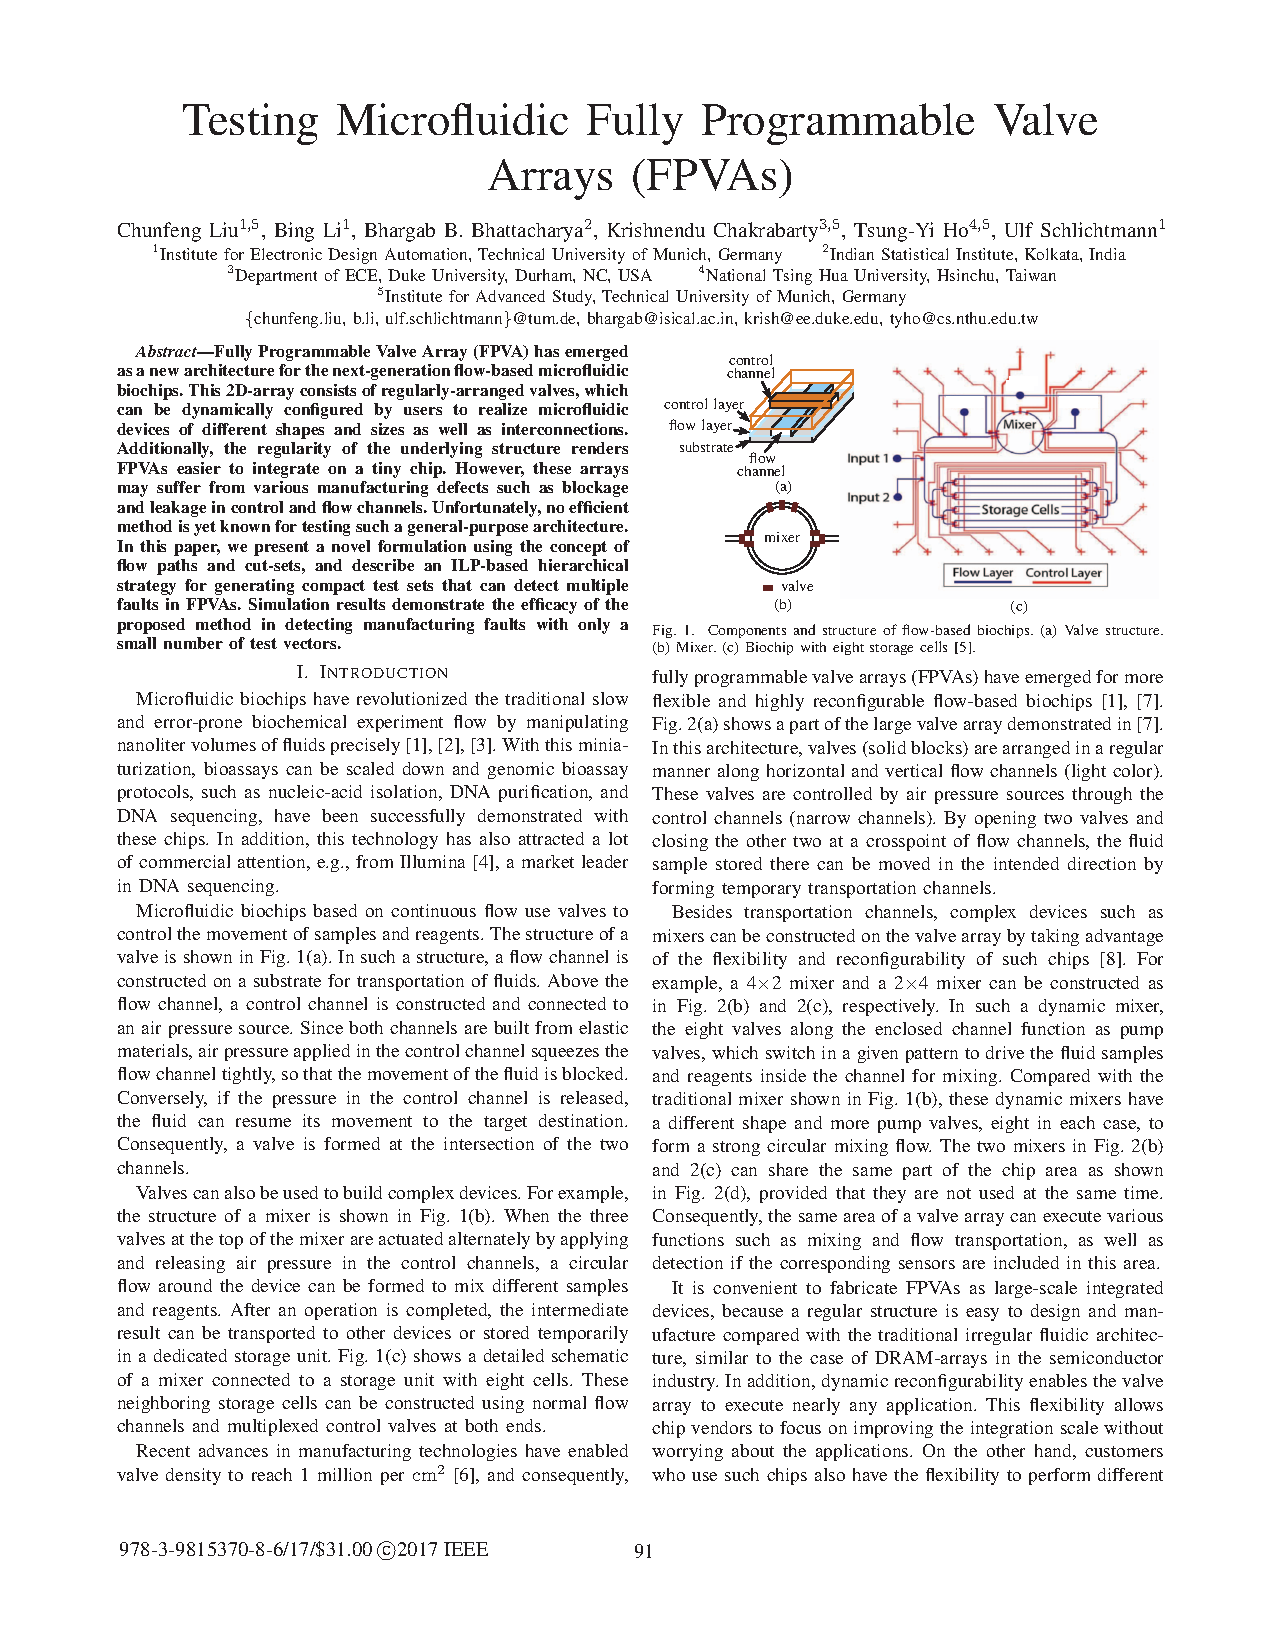
\includepdf[pages=1-last]{07926964.pdf}


\end{document}




